\section{Simultaneous optimization of multiple metrics is not always possible}\label{chapter:simultaneous_optimization}

Let \(\alpha_r \coloneqq \max\set{\tau' \mid \iconf{\tau}{r} = \iconf{t}{r}\ \forall \tau \geq \tau'}\) be the arrival time of \(r\), i.e.~the timestep when \(r\) stops moving.
Define \(P_r \coloneqq \set{ \parens{ \iconf{i}{r},\ \iconf{i + 1}{r} } \mid \parens{ \iconf{i}{r},\ \iconf{i + 1}{r} } \in E }\) to be the \emph{path} of \(r\): the sequence of steps \(r\) takes in a schedule. 

Then consider the following well-defined cost functions:
\begin{align*}
	% \smash and manual spacing to circumvent the larger block from \max_{r \in R}
	& \mono{Makespan} 				& \mono{(M)} && \schedules \mapsto \quad & \smash{\max_{r \in R}} \ \alpha_r 	\\[2mm] 
	& \mono{Total Arrival Time} 	& \mono{(TAT)} && \schedules \mapsto \quad & \Sigma_{r \in R} \ \alpha_r 		\\[2mm]
	& \mono{Total Distance} 		& \mono{(TD)} && \schedules \mapsto \quad & \Sigma_{r \in R} \ \abs{P_r} 		\\[2mm]
	& \mono{Maximum Distance} 		& \mono{(MD)} && \schedules \mapsto \quad & \max_{r \in R} \ \abs{P_r}
\end{align*}

% \cite{corr/YuL15c} examines all four of these on a general graph, i.e.~not contrained to model a grid like in our case. An important finding is proving the decision problem statements for the respective optimization problems of the cost functions above are all NP-complete on a general graph. This importantly does \emph{not} imply the same holds for the grid case of coordinated robot motion planning, and the reduction they use is not easily convertible to the grid. It seems currently unknown if the respective decision problems to these metrics are also NP-complete on the grid similar to \cref{thm:npc}.

\cite{corr/YuL15c} finds that for a robot motion planning problem on a \emph{general} graph, one cannot always find schedules that optimize any pair of the above cost functions simultaneously:
\begin{align}\label{eq:simultaneous_emptyset}
	\forall \parens{f_1,\ f_2} \in \set{\mono{M, TAT, TD, MD}}^2 : \exists I : \schedules_{\text{opt}_{f_1}} \cap \schedules_{\text{opt}_{f_2}} = \emptyset,
\end{align}
where \(\schedules_{\text{opt}_f} \subseteq \schedules\) denotes the set of optimal schedules for an instance \(I\) with respect to some cost function \(f\).
That \cref{eq:simultaneous_emptyset} is true on a general graph does not imply that it holds for our problem formulation on a grid, and the graphs used in the proof are not compatible with our grid-model.
However, by coming up with new grid-specific problem instances we prove the statement holds on the grid as well.

\begin{lemma}\label{lemma:simultaneous_pairings_1}
	A pairing of cost functions \(\parens{f_1, f_2} \in \set{\mono{M, MD}} \times \set{\mono{TAT, TD}}\) cannot always be simultaneously optimized on the grid.
\end{lemma}

\begin{proof}
	% FIGURE SIMULTANEOUS 1 PROBLEM
	\begin{figure}[h]
		\centering
		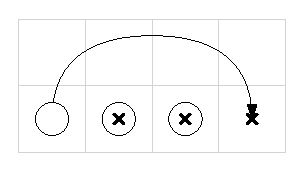
\includegraphics[width=0.35\linewidth]{ipe/sim1_problem.eps}
		\caption{
			A problem instance that requires different schedules depending on the cost function. Circles represent robots, crosses represent their targets. The two robots in the middle are already on their targets.
		}
		\label{fig:simultaneous_problem_1}
	\end{figure}

	Observe the configuration in \cref{fig:simultaneous_problem_1}. 
	It is easy to see that there are two different ways to schedule a solution: either sacrifice maximum time and distance by letting the single robot move around the two central ones, or alternatively let the middle robots move out of the way, sacrificing the total travel time and distance instead.
	See \cref{fig:simumtaneous_strategies_1} for a visual of this.

	% FIGURE SIMULTANEOUS 1 STRATEGIES
	\begin{figure}[h]
		\centering
		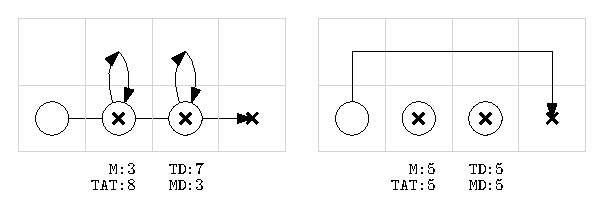
\includegraphics[width=0.7\linewidth]{ipe/sim1_strat.eps}
		\caption{
			The left schedule optimizes \mono{M}\ and \mono{MD}, while the right schedule optimizes \mono{TD}\ and \mono{TAT}.
		}
		\label{fig:simumtaneous_strategies_1}
	\end{figure}

It is quite trivial to conclude that there are no better solutions to this instance w.r.t. these metrics.
This implies one cannot always optimize simultaneously for any pairing in \(\set{\mono{M, MD}} \times \set{\mono{TAT, TD}}\) on the grid.
\end{proof}

\begin{lemma}\label{lemma:simultaneous_pairings_2}
	A pairing of cost functions \(\parens{f_1, f_2} \in \set{\mono{M, TAT}} \times \set{\mono{MD, TD}}\) cannot always be simultaneously optimized for on the grid.
\end{lemma}

\begin{proof}
	% FIGURE SIMULTANEOUS 2 PROBLEM
	\begin{figure}[h]
		\centering
		\includegraphics[width=0.45\linewidth]{ipe/sim2_problem.eps}
		\caption{
			A second instance that requires different schedules depending on the cost function.
		}
		\label{fig:simultaneous_problem_2}
	\end{figure}

	% FIGURE SIMULTANEOUS 2 STRATEGIES
	\begin{figure}[h]
		\centering
		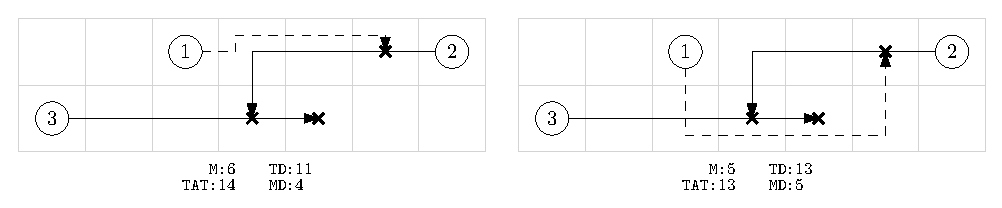
\includegraphics[width=\linewidth]{ipe/sim2_strat.eps}
		\caption{
			The left schedule optimizes \mono{TD}\ and \mono{MD}, while the right schedule optimizes \mono{M}\ and \mono{TAT}.
		}
		\label{fig:simultaneous_strategies_2}
	\end{figure}

	Similarly to \cref{lemma:simultaneous_pairings_1}, observe the instance in \cref{fig:simultaneous_problem_2}. 
	There are again two different strategies, seen in \cref{fig:simultaneous_strategies_2}: robot 1 either waits for robot 2 to pass, or alternatively goes a longer distance beneath robot 2.
	The instance is constructed so 2 and 3 have no choice but to move in these specific paths to avoid accumulating larger time and distance penalties, which means 1 has the only real choice here.
	As there are no better schedules than these for any of these metrics, it implies no schedule exists that optimizes the specific pairs in \cref{lemma:simultaneous_pairings_2} concurrently.
\end{proof}

\begin{theorem}
	A pair of cost functions \(\parens{f_1, f_2} \in \set{\mono{M, TAT, TD, MD}}^2 \) cannot always be simultaneously optimized for on the grid.
\end{theorem}

\begin{proof}
	\begin{figure}[h]
		\centering
		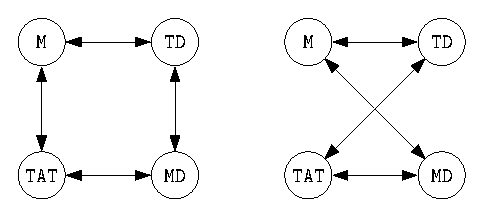
\includegraphics[width=0.5\textwidth]{ipe/sim_thm.eps}
		\caption{
			The pairs of sometimes simultaneously unoptimizable cost functions given \cref{lemma:simultaneous_pairings_1} and \cref{lemma:simultaneous_pairings_2} respectively.
		}
		\label{fig:simultaneous_pairings_graph}
	\end{figure}

	Consider the graphs in \cref{fig:simultaneous_pairings_graph} that show which cost functions are sometimes pairwise simultaneously unoptimizable.
	A new graph with the same vertices and a union of the edges clearly gives us a 4-clique, which is exactly what we are after.
	This implies the general proof from \cite{corr/YuL15c}, i.e.~\cref{eq:simultaneous_emptyset} also holds on the grid.
\end{proof}

The cost functions \emph{makespan}, \emph{total arrival time}, \emph{maximum distance} and \emph{total distance} are all natural ways to measure the cost of a schedule.
However, it is quite clear that optimizing for time-based metrics is more favorable than distance based ones when parallelism is desired.
Optimizing for distance traveled will clearly generate sequential schedules in some cases, completely disregarding the parallelism of the robots and taking an unreasonable amount of time to execute.

One could consider an extension of the \mono{TAT}\ metric, where the start times would be removed, i.e.~only summing the time from start to target.
Though one can again reason that these will again produce some sequential schedules similar to distance based metrics.

When considering motion planning for robots in warehouses, the biggest factor to consider is probably that multiple motion planning problems are to be executed in sequence, one after the other.
Making the schedules be independent of the previous and next schedules makes motion planning easily parallelizable: otherwise the starting times would be dependent on the previous arrival times and so on.
Makespan is specifically measuring the length of this independent schedule, which seems to make it a natural choice for a warehouse looking to utilize multiple robots.

% A completely sequential schedule wastes the parallel potential of multiple robots, and measuring only the distances traveled will make some optimal schedules have unreasonable makespans.



